\documentclass{article}
\pagenumbering{arabic} 
\usepackage{graphicx}
\usepackage[a4paper, portrait, total={6.5in, 9.6in}]{geometry}
\graphicspath{{./images/}}
\newcommand\tab[1][1cm]{\hspace*{#1}}

\usepackage{titlesec}

\titlespacing*{\section}
{0pt}{1ex}{1ex}

\usepackage{hyperref}
\hypersetup
{
	colorlinks=true,
	linkcolor=blue,
	filecolor=magenta,      
	urlcolor=cyan,
}
\urlstyle{same}

\usepackage{enumitem}
\setlist{nosep}

\begin{document}
	
	\begin{center}
		\huge\textbf{Chirag Shah}
	\end{center}
	
	\noindent
	\hrulefill
	%\newline
	\vskip .5cm
	\noindent \parbox[t]{0.7\linewidth}
	{
		16-Marina House, \\ 5-Sir V.T Marg, \\ Opp Liberty Cinema,\\ Mumbai 400 020 \\ Maharashtra
	}	 
	\vspace{.6cm}
	\parbox[t]{0.45\linewidth}
	{
		Contact: 9769168825 \\ chirags1998@gmail.com \\	\\	
		\tab 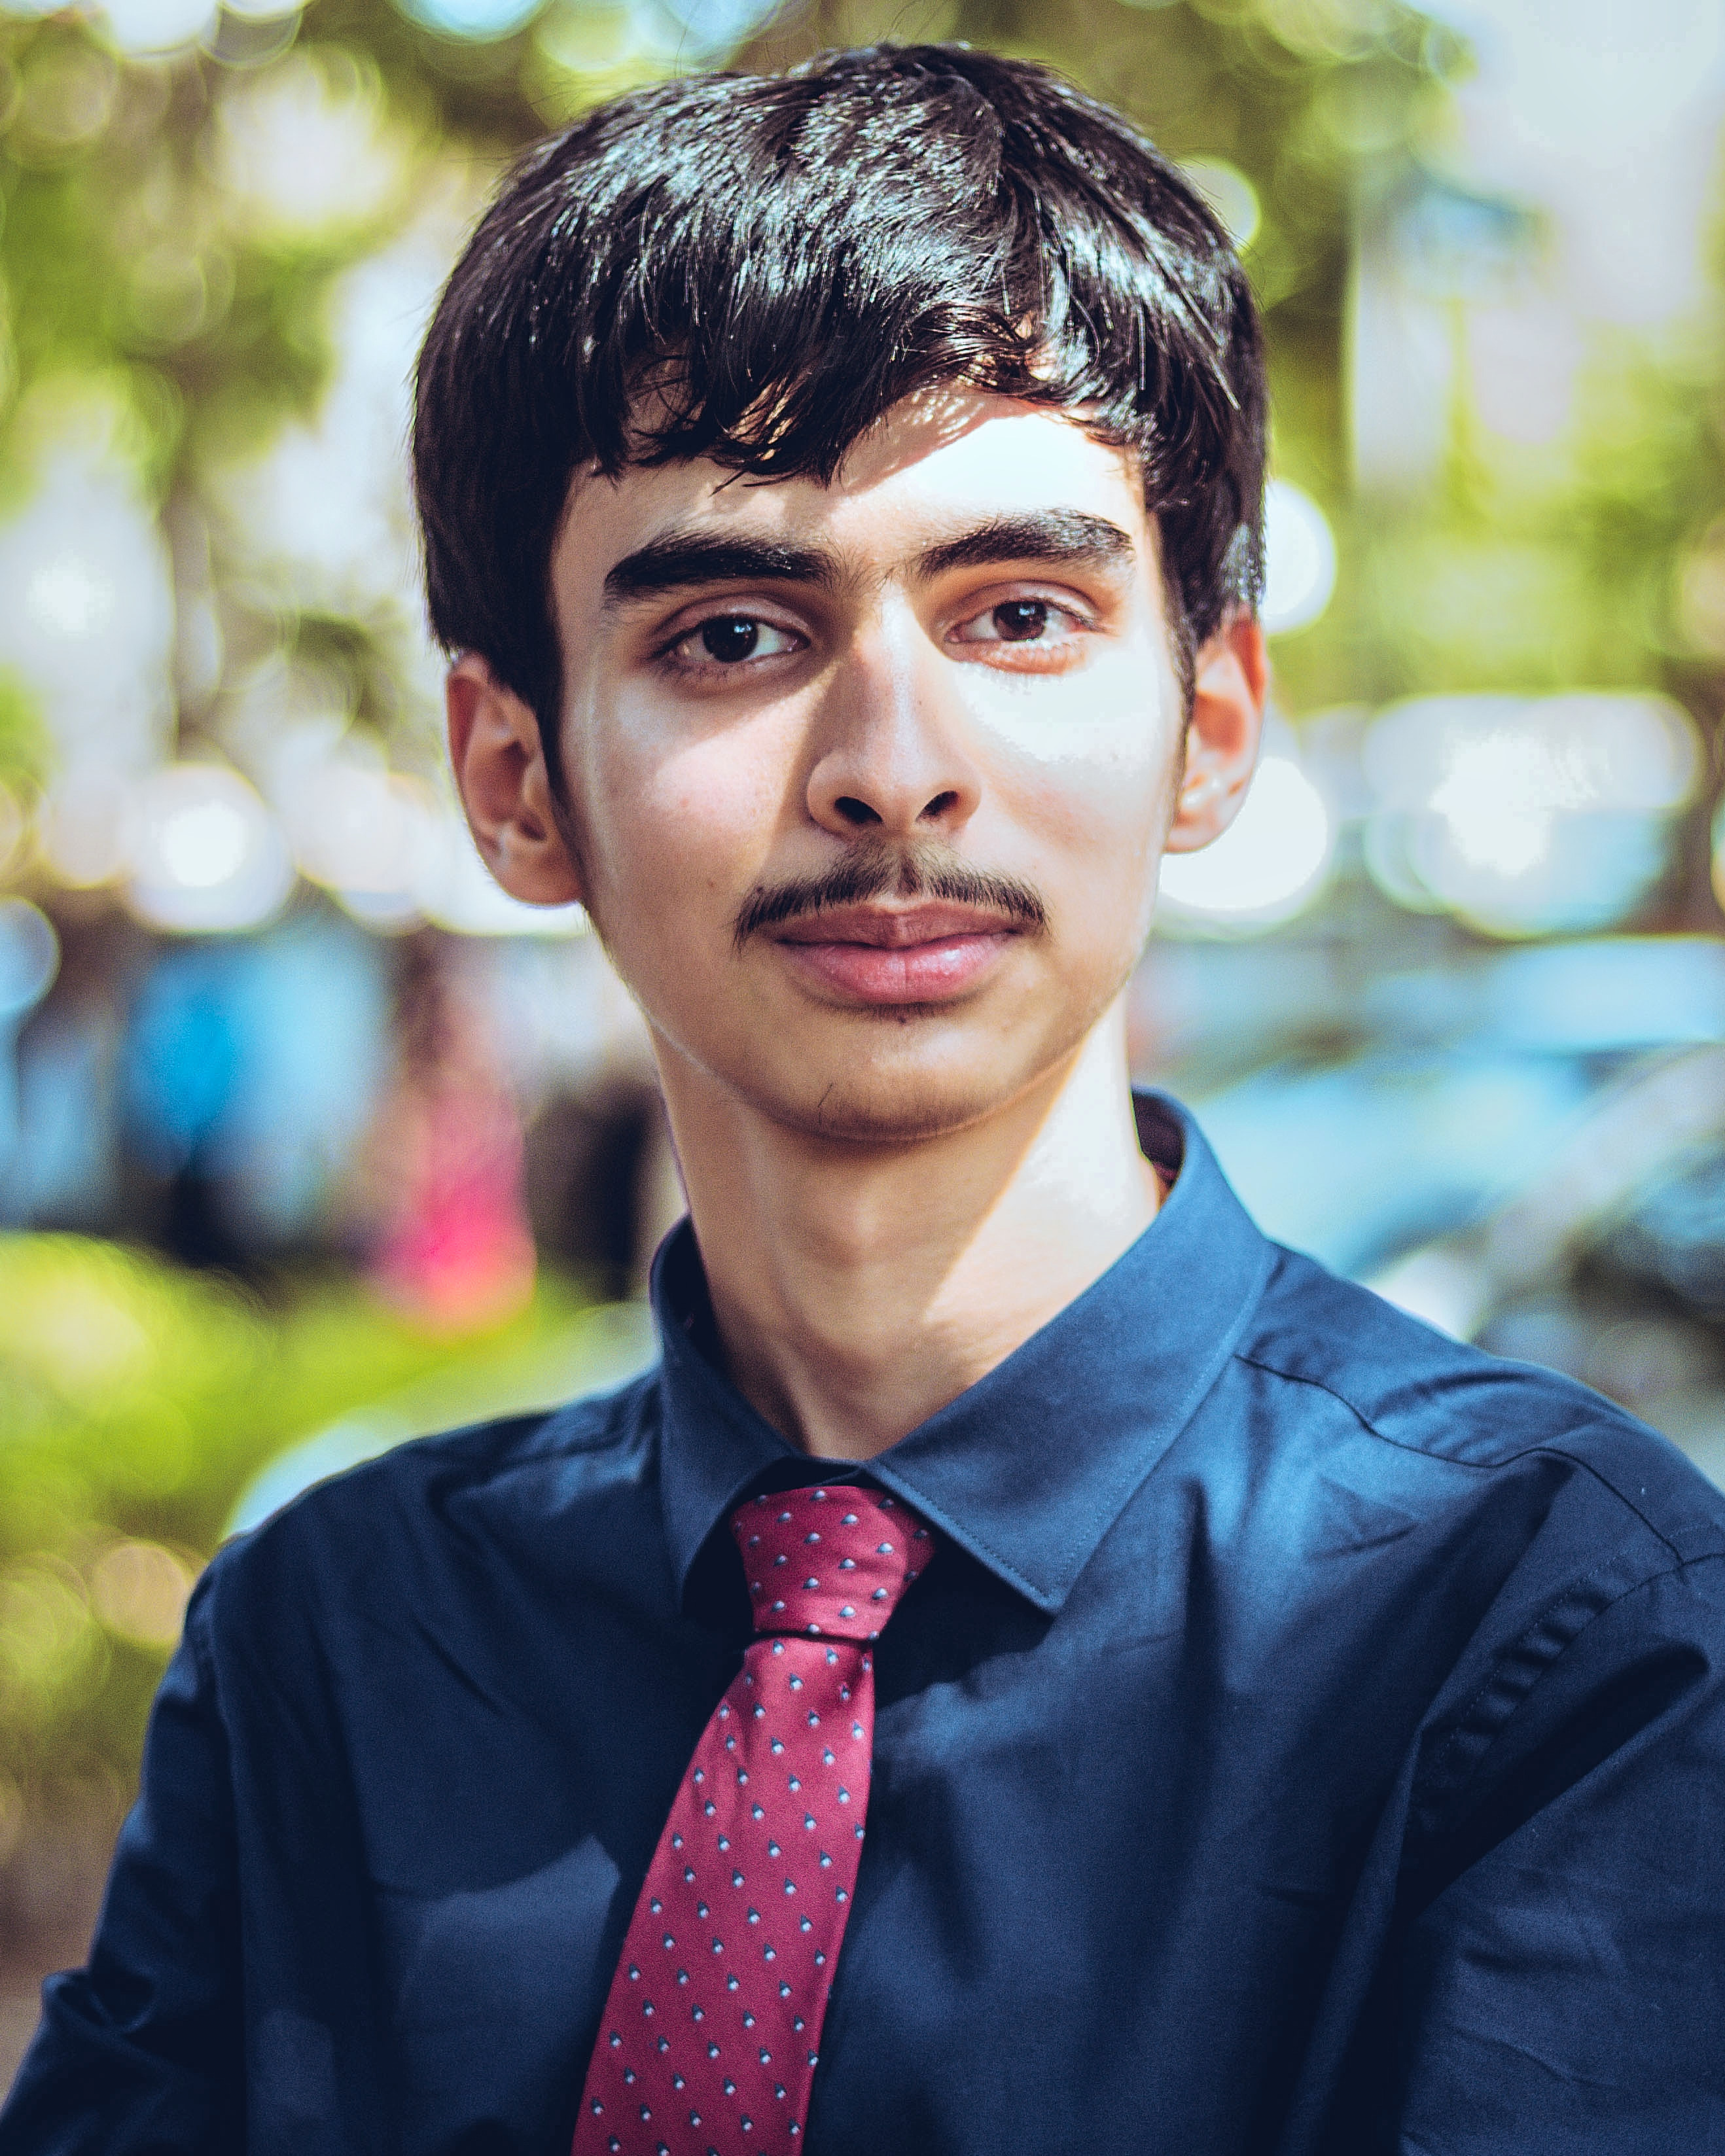
\includegraphics[scale =.115]{photo.jpg}
	}
	
	\section*{Career Objective}
	%To work as a system/product design engineer in the electronics industry where I can develop and apply my hardware and software skills
	To obtain a niche position in the Electronics industry where I can utilize my passion of combining both my hardware and software skills together and create a meaningful product for the organization
	
	\section*{Education}
	
	Currently studying in second year, Electronics Engineering, Sardar Patel Institute of Technology, Mumbai
	\newline
	\begin{tabular}{|c|c|c|c|c|}
		\hline
		Degree & College/School & University & Passing Year & Pass \% \\
		\hline
		HSC & PACE Junior Science College, Dadar & Maharashtra State Board & 2015 & 82.31\\
		\hline
		SSC & St Xaviers High School, Fort & Maharashtra State Board  & 2013 & 87.5\\
		\hline
	\end{tabular}
	
	\section*{Projects and Competitions}
	\begin{itemize}%[noitemsep]
		%\setlength\itemsep{-.1em}
		
		\item 1st position in \textbf{e-Yantra Robotics competition 2016}. \\
		Team was placed 1st out of 162 teams in the theme ``Launch a Module''  
		\verb|-| Incharge of hardware design and embedded C programming\\
		\url{http://eycgen.e-yantra.org/index.php/validate/fff9370353355910a5556b2d87c8e4b04f50a00d}		
		
		\item``\textbf{Formation Control of Multiple Swarm Robots}" project for eYantra Summer Internship 2017\\
		\url{https://github.com/eYSIP-2017/eYSIP-2017_Formation_Control_of_Multiple_Swarm_Robots}
			
		\item My project \textbf{DIY Timelapse Dolly} was featured and won the first prize in \textbf{The Raspberry Pi contest 2016} contest on Instructables out of 27 finalists from 198 entries\\
		\url{www.instructables.com/id/DIY-Time-Lapse-Dolly-1/}
		
		\item Won Second prize in Troubleshooting Competition organized by SPIT - Department of Electronics Engineering Mumbai from 29th/Sep /2016 to 17th/Oct/2016			
	\end{itemize}
	
	\section*{Internships}
	\begin{itemize}
		\item[$\bullet$] 7 weeks summer internship at IIT-Bombay under eYantra Summer Internship Program 2017
	\end{itemize} 
	
	\section*{Training}
	\begin{itemize}
		\item[$\bullet$] 7 weeks summer internship at IIT-Bombay under the eYantra Summer Internship 2017
		\item[$\bullet$] 3 weeks summer training program on Embedded Systems System Design held from 13/June/2016 to 8/July/2016 at SPIT College Mumbai
		\item[$\bullet$] 2 days workshop on MSP-FPGA Software and Hardware co-design conducted on 16th and 18th Sep 2016 at SPIT, Mumbai
	\end{itemize} 
		
	\section*{Technical Skills}
	\begin{itemize}
		\item[$\bullet$] Embedded C programming
		\item[$\bullet$] Project management using Git
		\item[$\bullet$] PCB designing and fabrication
		\item[$\bullet$] Good electronic hardware and circuit debugging skills
		\item[$\bullet$] Basic image processing using OpenCV and python
		\item[$\bullet$] Basic FPGA programming - Atlys Spartan-6 FPGA Trainer Board
		\item[$\bullet$] Document formatting using \LaTeX
	\end{itemize}
	
	\section*{Soft Skills}
	\begin{itemize}
		\item Patient and persistent in completing my projects
		\item Willing to learn new skills as per the requirements of the project
		\item Good analytical and problem solving skills
	\end{itemize}
	
	%\section*{Extra Curricular Activities}
	\section*{Other Interests}
	\begin{itemize}
		\item[$\bullet$] PADI Level 2 certified open water scuba diver
		\item[$\bullet$] Sailing and Wind surfing
		\item[$\bullet$] Rubik’s cube enthusiast 
		\item[$\bullet$] Photography 
	\end{itemize}
	
	\section*{Co-Curricular Activities}
	\begin{itemize}
		\item Class Representative\verb|:| FY \& SY (Electronics Engg) 
		\item Core Team Member of SPOpen Mini - 2016 (Speed cubing competition) \verb|-|Responsible for volunteer training.\\
		\url{www.worldcubeassociation.org/competitions/SPOpenMini2015}
	\end{itemize}
		
	\section*{References}
	\begin{enumerate}
		\item
		\begin{tabbing}
			Name: 		 \=Dr. Rita Das\\ 
			Desig: \>Dean, Students\verb|'| Affairs\\
			\>Associate Professor (Physics), Head of Applied Sciences \& Humanites Department,\\
			\>Sardar Patel Institute of Technology\\
			%Phone:\\ 
			Email: \>rita\_das@spit.ac.in\\ 
		\end{tabbing}
		
		\item
		\begin{tabbing}
			Name: 	 \=Prof. Govind Haldankar\\
			Desig:
			\>Assistant Professor, Electronics Engineering department,\\
			\>Sardar Patel Institute of Technology\\  
			%Phone:\\ 
			Email: \>g\_haldankar@spit.ac.in\\ 
		\end{tabbing}	
		
	\end{enumerate}
	
	\section*{Declaration}
	\tab I do hereby declare that the above given statements are true and correct to the best of my knowledge.\\
	
	\vspace{2cm} 
	\noindent \parbox[t]{0.7\linewidth}
	{
		\textbf{Place:} Mumbai\\
		\textbf{Date:} $24^{th}$ April 2017	
	}	 
	\vspace{0.15cm}
	\parbox[t]{0.45\linewidth}
	{
		\vspace{0.15cm}
		\textbf{Chirag Shah}
	}
	%\noindent
	%\hrulefill
	
\end{document}